% !TeX program = xelatex
\documentclass[a4paper]{article}

% ==================== FONT SETUP ====================
\usepackage{fontspec}
\usepackage{unicode-math}
\setmainfont{Times New Roman} % text font
\setmathfont{XITS Math}
\setsansfont{Arial} % sans font
\setmonofont{Consolas} % mono font


% ==================== PAGE LAYOUT ====================
\usepackage[left=30mm, top=25mm, right=20mm, bottom=25mm]{geometry}
\geometry{a4paper}

% ==================== LANGUAGE & CAPTION ====================
\renewcommand{\figurename}{Hình}

% ==================== FONT SIZE ====================
\usepackage{scrextend}
\changefontsizes{13pt}

% ==================== HEADER & FOOTER ====================
\usepackage{fancyhdr}
\pagestyle{fancy}
\lhead{\it PBL 1: Đồ án lập trình tính toán}
\rhead{\it Chương trình quản lý gia phả}
\lfoot{\it Nguyễn Đình Hải Đăng và Lê Bá Sơn}
\rfoot{Trang \thepage}
\cfoot{}
\renewcommand{\headrulewidth}{0.4pt}
\renewcommand{\footrulewidth}{0.4pt}

% ==================== GRAPHICS & DRAWING ====================
\usepackage{graphicx}
\usepackage{tikz}
\usetikzlibrary{calc}
\usetikzlibrary{er, trees, positioning, arrows.meta, shadows, backgrounds, shapes.geometric}
\usepackage{float}
\usepackage[font=small,labelfont=bf]{caption}
\captionsetup[figure]{font=small, labelfont=bf, justification=centering}

\tikzset{
    person/.style={rectangle, rounded corners=3pt, draw=blue!60, fill=blue!5, very thick, inner sep=6pt, font=\bfseries\footnotesize, drop shadow, align=center},
    pathA/.style={fill=red!30, draw=red!80},
    pathB/.style={fill=green!30, draw=green!80},
    LCA/.style={fill=yellow!40, draw=orange!90, line width=2pt},
    line/.style={-Stealth, thick, gray!80}
}

% ==================== MATH & ALGORITHM ====================
\usepackage{amsmath}
\usepackage{algorithm}
\makeatletter
\renewcommand{\ALG@name}{Mã giả}
\makeatother
\usepackage[noend]{algpseudocode}

% ==================== CODE LISTING ====================
\usepackage{listings}
\lstdefinestyle{cppstyle}{
	language=C++,
	basicstyle=\ttfamily\footnotesize,
	keywordstyle=\color{blue},
	commentstyle=\color{green!50!black},
	stringstyle=\color{red},
	numbers=none,
	showstringspaces=false,
	breaklines=true,
	frame=single,
	framesep=5pt,
	framerule=0.5pt
}
\lstdefinestyle{pseudostyle}{
	basicstyle=\ttfamily\footnotesize,
	numbers=none,
	showstringspaces=false,
	breaklines=true,
	frame=single,
	framesep=5pt,
	framerule=0.5pt,
}

% ==================== COLOR & BOXES ====================
\usepackage{xcolor}
\usepackage[breakable]{tcolorbox}
\usepackage{environ}
\usepackage{longtable}
\usepackage{array}

% ==================== HYPERLINKS ====================
\usepackage{hyperref}
\hypersetup{
	colorlinks,
	citecolor=blue,
	filecolor=blue,
	linkcolor=blue,
	urlcolor=blue
}

% ==================== TEXT FORMATTING ====================
\usepackage{setspace}
\setstretch{1.3}
\usepackage{parskip}
\setlength{\parindent}{0pt}
\usepackage{titlesec}
\titleformat{\section}
	{\normalfont\fontsize{14}{17}\bfseries}
	{\thesection.}{0.5em}{}
\titleformat{\subsection}
	{\normalfont\bfseries}
	{\thesubsection.}{0.5em}{}
\usepackage{enumitem}
\setlist[itemize]{noitemsep}
\setlist[enumerate]{noitemsep}

% ==================== UTILITIES ====================
\usepackage{verbatim}
\usepackage{lipsum}
\newcommand\HRule{\rule{\textwidth}{1pt}}
\usepackage{adjustbox}

% ==================== CUSTOM COMMANDS ====================
\let\oldalgorithmic\algorithmic
\let\endoldalgorithmic\endalgorithmic

\newcommand{\CodeFile}[1]{%
	\lstinputlisting[caption={#1}]{#1}%
}

\begin{document}
	\pagenumbering{roman}
	
\begin{tikzpicture}[remember picture, overlay]
		\draw[line width=3pt]
		($(current page.north west)+(2.7cm,-1.8cm)$)
		rectangle
		($(current page.south east)+(-1.8cm,1.8cm)$);
	\end{tikzpicture}
	
	\begin{center}
		\textbf{ĐẠI HỌC ĐÀ NẴNG} \\
		\textbf{TRƯỜNG ĐẠI HỌC BÁCH KHOA} \\
		{\large \textbf{KHOA CÔNG NGHỆ THÔNG TIN}}
	\end{center}
	
	\begin{figure}[h]
		\centering
		
\includegraphics[width=0.2\textwidth]{DUT-ITF-Logo.jpg} 
		%Lưu ý: Bạn cần thay thế 'logo.png' bằng đường dẫn đến tệp logo của bạn.
	\end{figure}
	
	\begin{center}
		\vspace{2cm}
		{\huge \textbf{ĐỒ ÁN LẬP TRÌNH TÍNH TOÁN}} \\
		{\LARGE \textbf{CHƯƠNG TRÌNH QUẢN LÝ GIA PHẢ}}
		\vspace{3cm}
	\end{center}
	
	\begin{center}
		{\large
		\makebox[0.8\textwidth][l]{\begin{tabular}{p{6.5cm}l}
				Giảng viên hướng dẫn: & \textbf{TS. Nguyễn Văn Hiệu} \\
				Sinh viên thực hiện: & \\
				\textbf{Nguyễn Đình Hải Đăng} & \textbf{Lớp: 25T\_KHDL} \\
				\textbf{Lê Bá Sơn} & \textbf{Lớp: 25T\_KHDL} \\
				\end{tabular}}
		}
	\end{center}
	
	\vfill
	
	\begin{center}
		{\large Đà Nẵng, tháng 6 năm 2026}
	\end{center}
	
	\thispagestyle{empty} 
	\clearpage
	
	% === TRANG 2: MỤC LỤC ===
	\newpage
    \thispagestyle{empty}
	\renewcommand{\contentsname}{MỤC LỤC}
	\tableofcontents
	
	% === TRANG 3: DANH MỤC HÌNH ẢNH ===
	\newpage
    \thispagestyle{empty}
	\renewcommand{\listfigurename}{}
	\begin{center}
		{\large \bfseries DANH MỤC HÌNH ẢNH}
	\end{center}
	\listoffigures
	\addcontentsline{toc}{section}{Danh mục hình ảnh}
	
	% === TRANG 6: NỘI DUNG CHÍNH ===
	\newpage
	\thispagestyle{empty}
	% Đánh số trang bắt đầu từ phần nội dung (tùy chọn, thường là trang 1)
	\setcounter{page}{1} 
	\pagenumbering{arabic}
	\addcontentsline{toc}{section}{Mở đầu}
	\begin{center}
		{\large \textbf{MỞ ĐẦU}}
	\end{center}
	
	\vspace{2\baselineskip}
	
	\leavevmode{\parindent=1em\indent} Trong bối cảnh công nghệ thông tin ngày càng phát triển mạnh mẽ, việc ứng dụng công nghệ vào giải quyết các bài toán thực tiễn đóng vai trò quan trọng. Trong đó, nhiều văn hoá truyền thống của dân tộc Việt Nam được ``số hoá'', tạo cơ hội cho những người trẻ - những người sống trong thời đại công nghệ được tiếp cận với truyền thống văn hoá nước nhà theo một cách mới mẻ và thú vị hơn.

\leavevmode{\parindent=1em\indent} Xuất phát từ ý tưởng số hóa và tổ chức thông tin về các mối quan hệ huyết thống trong gia đình, nhóm chúng em lựa chọn thực hiện đề tài \textbf{``Chương trình Quản lý gia phả''}. Mục tiêu của chương trình là xây dựng một hệ thống cho phép lưu trữ, quản lý và truy vấn thông tin các thành viên trong gia đình dưới dạng cấu trúc cây, từ đó hỗ trợ thực hiện các thao tác như thêm thành viên, tìm kiếm quan hệ họ hàng, duyệt cây gia phả và hiển thị thông tin một cách có hệ thống. Thông qua việc xây dựng chương trình, nhóm có cơ hội vận dụng các kiến thức cơ bản về cấu trúc dữ liệu, thuật toán và lập trình để giải quyết bài toán quản lý thông tin có cấu trúc phân cấp - đúng như tinh thần của phương pháp \textit{học tập qua dự án}.

\leavevmode{\parindent=1em\indent} Trong quá trình thực hiện dự án, nhóm đã nhận được sự hướng dẫn của TS. Nguyễn Văn Hiệu, giảng viên phụ trách học phần. Nhóm xin chân thành cảm ơn thầy đã định hướng và góp ý để nhóm có thể hoàn thành dự án này.

\leavevmode{\parindent=1em\indent} Mặc dù rất mong muốn thực hiện một chương trình hoàn chỉnh cả về nền tảng lý thuyết và phương pháp thực hiện, cũng như mong muốn có thêm phản hồi từ người dùng về chất lượng chương trình, tuy nhiên vì thời gian và trình độ còn hạn chế, vì vậy chương trình và báo cáo chắc chắn sẽ còn tồn tại những thiếu sót nhất định, kính mong quý thầy cô đóng góp ý kiến cho chương trình và báo cáo để nhóm rút kinh nghiệm cho những dự án PBL tiếp theo trong quá trình học tập tại trường.

\leavevmode{\parindent=1em\indent} Xin trân trọng cảm ơn.

	\newpage
	
	\section{TỔNG QUAN ĐỀ TÀI}
	
	Đề tài tập trung xây dựng một chương trình quản lý gia phả bằng ngôn ngữ C/C++, trong đó thông tin các thành viên và mối quan hệ huyết thống được mô hình hoá dưới dạng cấu trúc cây. Chương trình cho phép tạo lập, cập nhật, tra cứu và lưu trữ dữ liệu gia phả một cách có hệ thống.

Thông qua đề tài, sinh viên được rèn luyện kỹ năng phân tích bài toán thực tế, lựa chọn cấu trúc dữ liệu phù hợp và hiện thực hoá các chức năng cơ bản như thêm thành viên, duyệt cây và truy vấn quan hệ. Đề tài mang tính thực hành cao, phù hợp với mục tiêu của học phần PBL 1 và trình độ của sinh viên thực hiện.
	
	\section{CƠ SỞ LÝ THUYẾT}
	\subsection{Ý tưởng}
	Về cấu trúc dữ liệu cốt lõi, nhóm sử dụng Cấu trúc liên kết động (Dynamic Linked Structure). Mỗi thành viên trong gia phả được đại diện bởi một nút (Node) trong bộ nhớ Heap.

\textbf{Định nghĩa Nút (Person Node):} Mỗi nút chứa các thành phần thông tin cá nhân (Data) và các thành phần liên kết (Pointers).

\textbf{Cơ chế liên kết:} Nhóm sử dụng mô hình Left-Child Right-Sibling (LCRS) để biểu diễn cây đa phân, cụ thể:
\begin{itemize}
	\item \texttt{pLeftChild}: Con trỏ quản lý địa chỉ của người con đầu tiên.
	\item \texttt{pRightSibling}: Con trỏ quản lý địa chỉ của người em kế tiếp trong cùng một thế hệ.
	\item \texttt{pParent}: Con trỏ trỏ ngược về nút cha để tối ưu hóa thuật toán truy vết quan hệ (LCA).
\end{itemize}

Về quản lý bộ nhớ động, ý tưởng chính là tối ưu hóa tài nguyên hệ thống. Chỉ khi thêm một thành viên mới, chương trình mới sử dụng lệnh \texttt{new} để ``xin" cấp phát bộ nhớ. Điều này giúp hệ thống có thể quản lý gia phả với quy mô không giới hạn (tùy thuộc vào RAM) thay vì bị giới hạn bởi kích thước mảng khai báo trước. Ngoài ra, nhóm cài đặt cơ chế đệ quy để thu hồi bộ nhớ (\texttt{delete}) khi xóa một nhánh hoặc khi kết thúc chương trình, đảm bảo không xảy ra hiện tượng rò rỉ bộ nhớ (Memory Leak).

Về các thuật sử dụng trên cây con trỏ:
\begin{enumerate}
	\item Duyệt cây: Nhóm sử dụng thuật toán Duyệt theo chiều sâu (DFS) thông qua đệ quy để hiển thị sơ đồ gia phả. Việc di chuyển giữa các nút thực chất là việc truy cập vào địa chỉ bộ nhớ được lưu trữ trong các con trỏ liên kết.
	\item Định vị đối tượng: Thay vì tìm kiếm theo chỉ số (Index), nhóm xây dựng hàm tìm kiếm trả về địa chỉ vùng nhớ của đối tượng. Địa chỉ này sau đó được dùng làm tham số đầu vào cho các thao tác cập nhật hoặc thêm con cháu, giúp tốc độ truy cập dữ liệu đạt mức tối ưu.
\end{enumerate}
	\subsection{Cơ sở lý thuyết}
	\subsubsection{Cấu trúc dữ liệu cây}
Cây (Tree) là một cấu trúc dữ liệu phi tuyến tính, được sử dụng để biểu diễn các mối quan hệ phân cấp giữa các đối tượng. Trong cấu trúc cây, mỗi phần tử được gọi là một nút (node), các nút được liên kết với nhau thông qua quan hệ cha - con. Một cây có các đặc điểm cơ bản sau:
\begin{itemize}
	\item Có một nút gốc (root), là nút không có cha.
	\item Mỗi nút (trừ nút gốc) có duy nhất một nút cha.
	\item Mỗi nút có thể có không hoặc nhiều nút con.
	\item Không tồn tại chu trình trong cấu trúc cây.
\end{itemize}

Nhờ đặc tính phân cấp rõ ràng, cấu trúc cây đặc biệt phù hợp để mô hình hoá các hệ thống có quan hệ thứ bậc như cây thư mục, sơ đồ tổ chức, và gia phả.

Trong bài toán quản lý gia phả, mỗi thành viên trong gia đình được biểu diễn bởi một nút trong cây, trong đó:
\begin{itemize}
	\item Quan hệ cha-con tương ứng với quan hệ giữa các nút.
	\item Các thế hệ trong gia đình tương ứng với các mức (level) khác nhau của cây.
	\item Tổ tiên cao nhất được xem là nút gốc của cây gia phả.
\end{itemize}

Cách biểu diễn này cho phép mô hình hoá một cây nhiều nhánh với số lượng con bất kỳ, đồng thời đảm bảo cấu trúc dữ liệu gọn nhẹ, linh hoạt và thuận tiện cho việc cài đặt các thuật toán duyệt cây, thêm hoặc mở rộng gia phả trong ngôn ngữ C++.

\subsubsection{Biểu diễn cây bằng mô hình con đầu - anh em kế tiếp}

Đối với cây nhiều nhánh, mỗi nút có thể có số lượng nút con không xác định. Nếu lưu trực tiếp danh sách con cho mỗi nút, cấu trúc dữ liệu sẽ trở nên phức tạp và khó quản lý. Để khắc phục vấn đề này, đề tài sử dụng mô hình con đầu-anh em kế tiếp (first-child / next-sibling) để biểu diễn cây gia phả.

Trong mô hình này, mỗi nút trong cây chỉ cần hai liên kết chính:
\begin{itemize}
	\item Con trỏ \texttt{firstChild}: trỏ tới nút con đầu tiên của nút hiện tại.
	\item Con trỏ \texttt{nextSibling}: trỏ tới nút anh/chị/em kế tiếp có cùng nút cha.
\end{itemize}

Ngoài ra, mỗi nút còn lưu con trỏ parent trỏ tới nút cha, giúp việc truy vấn quan hệ cha - con và di chuyển ngược trong cây trở nên thuận tiện.

Với cách biểu diễn này:
\begin{itemize}
	\item Nếu một nút không có con, con trỏ \texttt{firstChild} có giá trị \texttt{nullptr}.
	\item Nếu một nút là người con cuối cùng, con trỏ \texttt{nextSibling} có giá trị \texttt{nullptr}.
	\item Các con của cùng một nút cha được liên kết thành một danh sách liên kết đơn thông qua \texttt{nextSibling}.
\end{itemize}

\begin{figure}[h]
	\centering
	\captionsetup{justification=centering}
	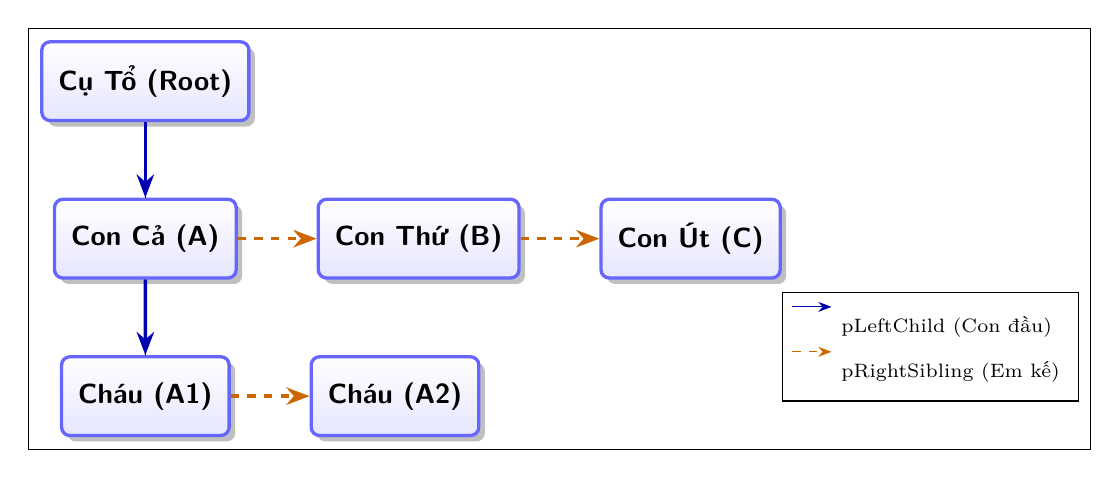
\begin{tikzpicture}[
		% Định nghĩa phong cách cho các nút (Node)
		person/.style={
			rectangle, 
			rounded corners=3pt, 
			draw=blue!60, 
			top color=white, 
			bottom color=blue!10,
			very thick, 
			inner sep=6pt, 
			minimum size=1cm, 
			font=\sffamily\bfseries,
			drop shadow
		},
		% Đường nối đến con đầu tiên (First Child)
		child-line/.style={
			-Stealth, 
			thick, 
			blue!70!black,
			line width=1.2pt
		},
		% Đường nối đến em kế tiếp (Next Sibling)
		sibling-line/.style={
			-Stealth, 
			dashed, 
			orange!80!black, 
			line width=1.2pt
		},
		% Cấu trúc cây
		level distance=2cm,
		sibling distance=2.5cm,
		show background rectangle, background rectangle/.style={draw=black}
		]
		
		% Vẽ các Node
		\node (root) [person] {Cụ Tổ (Root)}
		child {
			node (child1) [person] {Con Cả (A)}
			child {
				node (grandchild1) [person] {Cháu (A1)}
				child [missing] % Chỗ này để trống để tạo khoảng cách
			}
		};
		
		% Các nút anh em (Next Sibling) nằm ngang hàng
		\node (child2) [person, right=of child1] {Con Thứ (B)};
		\node (child3) [person, right=of child2] {Con Út (C)};
		\node (grandchild2) [person, right=of grandchild1] {Cháu (A2)};
		
		% Vẽ các mũi tên First Child (Màu xanh, nét liền)
		\draw [child-line] (root.south) -- (child1.north) node[midway, left, font=\scriptsize, blue]{};
		\draw [child-line] (child1.south) -- (grandchild1.north) node[midway, left, font=\scriptsize, blue]{};
		
		% Vẽ các mũi tên Next Sibling (Màu cam, nét đứt)
		\draw [sibling-line] (child1.east) -- (child2.west) node[midway, above, font=\scriptsize, orange]{};
		\draw [sibling-line] (child2.east) -- (child3.west) node[midway, above, font=\scriptsize, orange]{};
		\draw [sibling-line] (grandchild1.east) -- (grandchild2.west) node[midway, above, font=\scriptsize, orange]{};
		
		% Chú thích (Legend)
		\matrix [draw, below right, xshift=0cm, yshift=-3.2cm] at (current bounding box.north east) {
			\draw [child-line, thin] (0,0) -- (0.5,0); & \node [font=\scriptsize] {pLeftChild (Con đầu)}; \\
			\draw [sibling-line, thin] (0,0) -- (0.5,0); & \node [font=\scriptsize] {pRightSibling (Em kế)}; \\
		};
		
	\end{tikzpicture}
	\caption{Hình minh hoạ mô hình biểu diễn cây theo cấu trúc con đầu - anh em kế tiếp}
	\label{fig:hinh1}
\end{figure}

Trong chương trình, mỗi thành viên trong gia phả được biểu diễn bởi một cấu trúc \texttt{Person}, trong đó các mối quan hệ được quản lý hoàn toàn bằng con trỏ. Việc thêm một người con mới được thực hiện bằng cách:
\begin{itemize}
	\item Nếu người cha chưa có con, gán trực tiếp nút mới cho \texttt{firstChild}.
	\item Nếu người cha đã có con, duyệt danh sách các con thông qua \texttt{nextSibling} để tìm người con cuối cùng (con út), sau đó nối nút mới vào cuối danh sách.
\end{itemize}

\begin{figure}[htbp]
	\vspace*{-\baselineskip}
	\centering
	\begin{algorithm}[H]
		\footnotesize
		\caption{Thêm con vào danh sách anh chị em}
		\begin{algorithmic}[1]
			\State child $\gets$ \Call{TaoDoiTuong}{Person, name, gender, parent}
			\If{parent.firstChild = null} \Comment{Nếu parent chưa có con đầu}
			\State parent.firstChild $\gets$ child \Comment{Gán child làm con đầu tiên của parent}
			\Else
			\State current $\gets$ parent.firstChild
			\While{current.nextSibling $\neq$ null}
			\State current $\gets$ current.nextSibling
			\EndWhile
			\State current.nextSibling $\gets$ child \Comment{Nối child vào cuối danh sách con của parent}
			\EndIf
		\end{algorithmic}
	\end{algorithm}
	\vspace*{-\baselineskip}
	\caption{Mã giả mô tả thuật toán thêm một người con vào cây gia đình}
	\label{fig:themCon}
	\vspace*{-\baselineskip}
\end{figure}
Cách biểu diễn này mang lại các ưu điểm sau:
\begin{enumerate}
	\item Biểu diễn được cây gia phả có số lượng con không giới hạn cho mỗi thành viên.
	\item Cấu trúc dữ liệu gọn nhẹ, mỗi nút chỉ cần số lượng con trỏ cố định.
	\item Thuận tiện cho việc duyệt cây theo chiều sâu và cài đặt các thuật toán xử lý quan hệ huyết thống.
	\item Phù hợp với việc rèn luyện kỹ năng sử dụng con trỏ và quản lý bộ nhớ động trong C++.
\end{enumerate}

Nhờ những đặc điểm trên, mô hình con đầu - anh em kế tiếp sử dụng con trỏ là lựa chọn phù hợp để hiện thực chương trình quản lý gia phả trong phạm vi đề tài.

\subsubsection{Duyệt cây và quản lý bộ nhớ}
Trong chương trình, việc xử lý và hiển thị gia phả được thực hiện thông qua duyệt cây theo chiều sâu, cụ thể là duyệt tiền thứ tự. Theo cách duyệt này, mỗi nút được xử lý trước, sau đó lần lượt duyệt đến nút con đầu tiên thông qua con trỏ \texttt{firstChild}, và tiếp tục duyệt các nút anh/chị/em kế tiếp thông qua con trỏ \texttt{nextSibling}.

Cách duyệt này rõ ràng phù hợp với mô hình con đầu - anh em kế tiếp và cho phép hiển thị gia phả theo thứ tự từ tổ tiên đến các thế hệ sau, phản ánh đúng cấu trúc phân cấp của gia đình.

Do chương trình sử dụng cấp phát bộ nhớ động cho các nút trong cây, việc quản lý và giải phóng bộ nhớ là yêu cầu bắt buộc. Khi kết thúc chương trình, toàn bộ các nút trong cây được giải phóng bằng một hàm đệ quy, đảm bảo không xảy ra rò rỉ bộ nhớ. Việc kết hợp duyệt cây và quản lý bộ nhớ động giúp chương trình hoạt động ổn định và an toàn trong môi trường C++.

\begin{figure}[h]
\begin{lstlisting}[style=cppstyle]
// Depth-First Traversal
void DisplayTree(Person* current, int level) {
	if (current == nullptr) return;
	// Child
	DisplayTree(current->firstChild, level + 1);
	// Sibling
	DisplayTree(current->nextSibling, level);
}

// Free up memory
void FreeTree(Person* current) {
	if (current == nullptr) return;
	FreeTree(current->firstChild);
	FreeTree(current->nextSibling);
	delete current;
}
\end{lstlisting}
\caption{Đoạn mã C++ thể hiện logic duyệt cây theo chiều sâu và giải phóng bộ nhớ.}
\label{fig:DfsAndFree}
\end{figure}

Đến đây, những cơ sở lý thuyết đã được trình bày ở trên đã căn bản làm nền tảng cho toàn bộ quá trình thiết kế chương trình sau này.
	
	\section{TỔ CHỨC CẤU TRÚC DỮ LIỆU VÀ THUẬT TOÁN}
	\subsection{Phát biểu bài toán}
Trong việc quản lý gia phả của một dòng họ, thách thức lớn nhất nằm ở tính phân cấp và sự biến động của dữ liệu. Cụ thể, bài toán đặt ra các yêu cầu và ràng buộc sau:
\begin{itemize}
	\item Thứ nhất, một cá nhân có thể là con của người này nhưng lại là cha/mẹ của người khác. Mối quan hệ này kéo dài qua nhiều thế hệ, tạo thành một cấu trúc cây.
	\item Thứ hai, khác với cây nhị phân (mỗi nút chỉ có tối đa 2 con), một người trong thực tế có thể có số lượng con bất kỳ. Việc sử dụng mảng cố định để lưu trữ danh sách con sẽ gây lãng phí bộ nhớ hoặc thiếu linh hoạt.
	\item Thứ ba, cần lưu trữ rõ ràng các thông tin thực thể (Tên, giới tính, ngày sinh...) và các mối quan hệ (Cha-con, Anh-chị-em).
	\item Cuối cùng, bài toán yêu cầu các thao tác: thêm mới, duyệt và tìm kiếm.
\end{itemize}
\subsection{Cấu trúc dữ liệu}
\subsubsection{Thiết kế chung}

Để giải quyết bài toán quản lý thông tin đa dạng của mỗi cá nhân trong dòng họ, chương trình thiết kế một kiểu dữ liệu tự định nghĩa (\texttt{struct person}). Sơ đồ cấu trúc được mô tả ở Hình \ref{fig:ERD1}. Cấu trúc này ánh xạ trực tiếp các yêu cầu của thực tế vào không gian bộ nhớ:
\begin{itemize}
	\item Nhóm thuộc tính định danh và nhân khẩu học: Các trường dữ liệu \texttt{name}, \texttt{gender}, \texttt{birthday}, \texttt{job} được sử dụng để lưu trữ hồ sơ cơ bản. Trong đó, \texttt{gender} (Nam/Nữ) đóng vai trò là cờ điều hướng (flag) để quyết định cấu trúc phát triển của cây; trường \texttt{birthday} đóng vai trò định hình thứ tự anh - em trong những người con của cùng một cha.
	\item Nhóm thuộc tính gia đình và tình trạng: Trường \texttt{spouseName} (Tên vợ/chồng) được gắn trực tiếp như một thuộc tính của Nút thay vì tạo một Nút độc lập, giúp giảm độ phức tạp của đồ thị cây. Ngoài ra, kỹ thuật này đảm bảo cấu trúc gia phả luôn là một cây đơn gốc, giúp duy trì tính toàn vẹn cho các thuật toán đệ quy và tìm tổ tiên chung (LCA) mà không làm tăng độ phức tạp của đồ thị thành dạng chu trình. Trường deathDay quản lý tình trạng sinh tử, và \texttt{numChildren} (số con) được thiết kế đặc biệt chỉ kích hoạt lưu trữ đối với thành viên Nữ. 
	\item Nhóm thuộc tính định tuyến (Routing Attributes): Các con trỏ \texttt{pParent}, \texttt{pFir-stChild}, \texttt{pNextSibling} đóng vai trò là ``chỉ dẫn đường" để móc nối thực thể này vào mạng lưới gia phả chung, đảm bảo tính liên kết động mà không cần mảng trung gian.
\end{itemize}
\begin{figure}[!h]
	\centering
    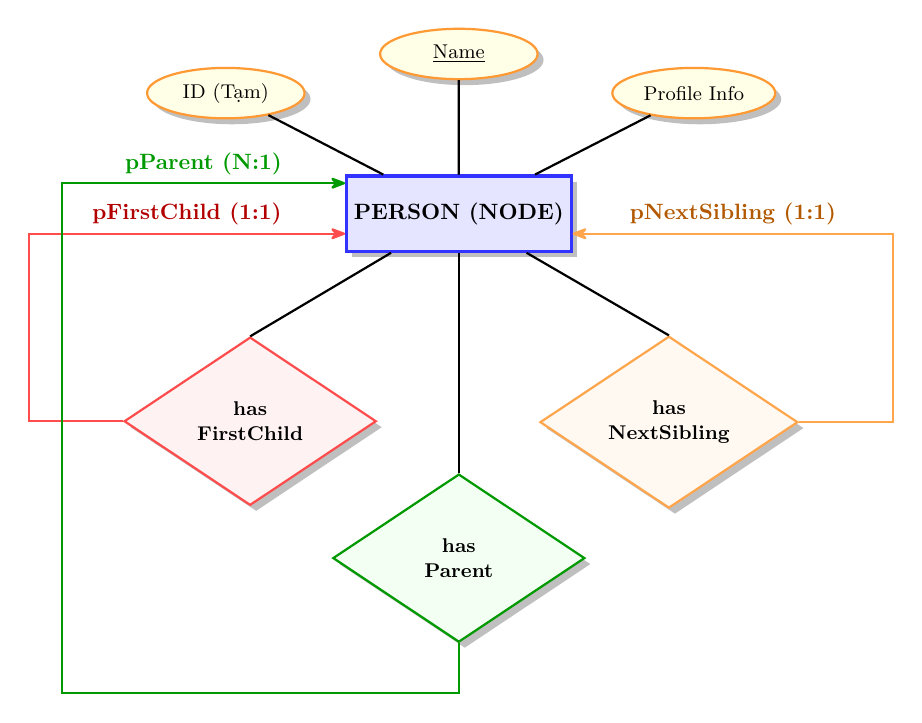
\begin{tikzpicture}[
    node distance=2.5cm,
    transform shape,
    % Tự định nghĩa lại các khối đồ họa cơ bản nhất
    entity/.style={
        rectangle, draw=blue!80, fill=blue!10, 
        very thick, minimum width=3.5cm, minimum height=1.2cm, 
        font=\bfseries, drop shadow
    },
    attribute/.style={
        ellipse, draw=orange!80, fill=yellow!10, 
        thick, minimum width=2.5cm, minimum height=0.8cm, 
        font=\small, drop shadow
    },
    relationship/.style={
        diamond, draw=gray!80, fill=gray!10, 
        thick, aspect=1.5, text width=2.5cm, align=center,
        font=\small\bfseries, drop shadow
    },
    >={Stealth[round]},
    scale=0.8
]

    % 1. THỰC THỂ TRUNG TÂM
    \node[entity] (person) {PERSON (NODE)};

    % 2. CÁC THUỘC TÍNH (Gộp bớt để sơ đồ thoáng)
    \node[attribute] (name) [above=1.5cm of person] {\underline{Name}} edge[thick] (person);
    \node[attribute] (info) [above right=1cm and 1cm of person] {Profile Info} edge[thick] (person);
    \node[attribute] (id) [above left=1cm and 1cm of person] {ID (Tạm)} edge[thick] (person);

    % 3. QUAN HỆ FIRST CHILD (Màu đỏ, vòng về bên trái)
    \node[relationship, draw=red!70, fill=red!5] (rc) [below left=2cm and 0.5cm of person] {has\\FirstChild};
    \draw[-, thick] (person.210) -- (rc.north);
    \draw[->, red!70, thick] (rc.west) -- ++(-1.5,0) |- (person.190) 
        node[pos=0.75, above, font=\bfseries, text=red!70!black] {pFirstChild (1:1)};

    % 4. QUAN HỆ NEXT SIBLING (Màu cam, vòng về bên phải)
    \node[relationship, draw=orange!70, fill=orange!5] (rs) [below right=2cm and 0.5cm of person] {has\\NextSibling};
    \draw[-, thick] (person.330) -- (rs.north);
    \draw[->, orange!70, thick] (rs.east) -- ++(1.5,0) |- (person.350) 
        node[pos=0.75, above, font=\bfseries, text=orange!70!black] {pNextSibling (1:1)};

    % 5. QUAN HỆ PARENT (Màu xanh, vòng cung rộng ôm trọn bên trái)
    \node[relationship, draw=green!60!black, fill=green!5] (rp) [below=3.5cm of person] {has\\Parent};
    \draw[-, thick] (person.270) -- (rp.north);
    % Vẽ đường Parent vòng xa ra ngoài để không đè lên FirstChild
    \draw[->, green!60!black, thick] (rp.south) -- ++(0,-0.8) -| ([xshift=-4.5cm]person.west) |- (person.165) 
        node[pos=0.75, above, font=\bfseries, text=green!60!black] {pParent (N:1)};

\end{tikzpicture}
\caption{Sơ đồ ERD mô tả thực thể Person và các mối quan hệ tự thân trong cấu trúc cây LCRS}
\label{fig:ERD1}
\end{figure}



\subsubsection{Cài đặt các ràng buộc cần thiết}
Cấu trúc dữ liệu đã được tùy biến để tuân thủ nghiêm ngặt các quy tắc truyền thống của một gia phả dòng họ, gồm hai ý chính:
\begin{enumerate}
	\item Theo yêu cầu đề tài, con gái khi lập gia đình sẽ tính theo gia phả nhà chồng. Do đó, trong giải thuật \texttt{AddChild} (Thêm con), nhóm đã cài đặt chốt chặn logic, nghĩa là: Khi người dùng thực hiện thao tác thêm thế hệ mới, chương trình sẽ kiểm tra \texttt{parent->gender}. Nếu giá trị là ``Nữ", thao tác bị từ chối và nút đó vĩnh viễn là một ``Nút lá" (không bao giờ có \texttt{pFirstChild}).
	\item Trong một dòng họ, việc trùng họ tên giữa các thế hệ là khá phổ biến (ví dụ: nhiều người cùng tên ``Nguyễn Văn A"). Việc tìm kiếm và cập nhật của chương trình nếu chỉ dựa vào chuỗi name sẽ dẫn đến sai lệch nghiêm trọng. Để giải quyết, nhóm cơ chế Lọc danh sách lựa chọn (Selection List). Thay vì định danh bằng chuỗi ký tự không duy nhất, chương trình sử dụng địa chỉ bộ nhớ làm định danh tuyệt đối, kết hợp với việc truy vấn thuộc tính phụ từ người dùng để xác nhận đối tượng.
\end{enumerate}

\subsection{Thuật toán và đánh giá thuật toán}
\subsubsection{Thuật toán Duyệt và Tìm kiếm}

Vì các nút bộ nhớ (\texttt{Person}) được cấp phát động trên RAM, chương trình thiết kế hai chiến lược truy vấn chuyên biệt dựa trên loại khóa tìm kiếm để tối ưu hóa hiệu năng hệ thống:

\textbf{Truy vấn theo Định danh (ID Lookup)}
	\begin{itemize}
		\item \textit{Cơ sở lý thuyết:} Sử dụng cấu trúc Bảng băm (Hash Table) nhằm thiết lập ánh xạ trực tiếp $f: ID \rightarrow \text{Memory Address}$, cho phép truy xuất dữ liệu độc lập với độ sâu của đồ thị cây.
		\item \textit{Phương pháp thực hiện:} Kỹ thuật này được kích hoạt trong tiến trình đọc tệp nhị phân \texttt{.dat}. Chương trình khởi tạo \texttt{std::unordered\_map<int, Person*>} để lưu trữ danh sách các nút vừa cấp phát. Khi cần khôi phục tập hợp cạnh $E$ (nối con trỏ cha-con), hệ thống chỉ cần truyền \texttt{parentId} vào Bảng băm để nhận lại con trỏ thực thi ngay lập tức. Hình \ref{fig:Hash1} mô tả dễ hiểu quá trình này.
		\item \textit{Phân tích độ phức tạp:} Thuật toán đưa độ phức tạp thời gian tìm kiếm cha từ $O(|V|)$ xuống $O(1)$ tuyệt đối, giải quyết triệt để nút thắt cổ chai khi hệ thống phải tái thiết lập hàng vạn liên kết con trỏ.
	\end{itemize}

\vspace{0.5cm}
	
\begin{figure}[h!]
	\vspace*{-\baselineskip}
	\centering
	\begin{adjustbox}{center=-3cm}
	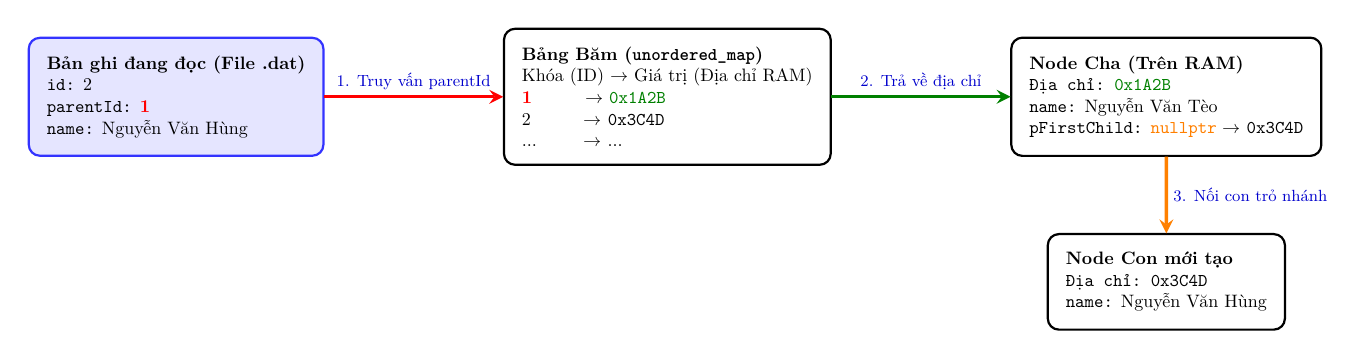
\begin{tikzpicture}[
		>=stealth, thick,
		box/.style={draw=black, fill=white, rounded corners, inner sep=10pt, align=left},
		highlight/.style={draw=blue!80, fill=blue!10, thick},
		arrowtext/.style={midway, above, font=\scriptsize\itshape, text=blue!80!black},
		transform shape,
		scale=0.65
		]
		
		\node[box, highlight] (file) {
			\textbf{Bản ghi đang đọc (File .dat)}\\
			\texttt{id:} 2 \\
			\texttt{parentId:} \textcolor{red}{\textbf{1}} \\
			\texttt{name:} Nguyễn Văn Hùng
		};
		
		% Khối 2: Bảng Băm (Hash Table)
		\node[box, right=3.5cm of file] (hash) {
			\textbf{Bảng Băm (\texttt{unordered\_map})}\\
			Khóa (ID) $\rightarrow$ Giá trị (Địa chỉ RAM)\\
			\textcolor{red}{\textbf{1}} \hspace{0.8cm} $\rightarrow$ \textcolor{green!50!black}{\texttt{0x1A2B}} \\
			2 \hspace{0.8cm} $\rightarrow$ \texttt{0x3C4D} \\
			... \hspace{0.6cm} $\rightarrow$ ...
		};
		
		% Khối 3: Cây LCRS trên RAM
		\node[box, right=3.5cm of hash] (ram_parent) {
			\textbf{Node Cha (Trên RAM)}\\
			\texttt{Địa chỉ: }\textcolor{green!50!black}{\texttt{0x1A2B}} \\
			\texttt{name:} Nguyễn Văn Tèo \\
			\texttt{pFirstChild:} \textcolor{orange}{\texttt{nullptr}} $\rightarrow$ \texttt{0x3C4D}
		};
		
		\node[box, below=1.5cm of ram_parent] (ram_child) {
			\textbf{Node Con mới tạo}\\
			\texttt{Địa chỉ: 0x3C4D} \\
			\texttt{name:} Nguyễn Văn Hùng
		};
		
		% Vẽ mũi tên liên kết
		\draw[->, red, very thick] (file.east) -- (hash.west) node[arrowtext, font=\small] {1. Truy vấn parentId};
		\draw[->, green!50!black, very thick] (hash.east) -- (ram_parent.west) node[arrowtext, font=\small] {2. Trả về địa chỉ};
		\draw[->, orange, very thick] (ram_parent.south) -- (ram_child.north) node[arrowtext, right, font=\small] {3. Nối con trỏ nhánh};
		
	\end{tikzpicture}
\end{adjustbox}
	\caption{Mô phỏng quy trình thực hiện truy vấn theo Định danh bằng cấu trúc Bảng băm}
	\label{fig:Hash1}
\end{figure}


\begin{figure}[H]
	\vspace*{-\baselineskip}
	\centering
	\begin{minipage}{0.50\textwidth}
		\begin{algorithm}[H]
			\footnotesize
			\caption*{Pha 1: Cấp phát nút}
			\begin{algorithmic}
				\State Khởi tạo bảng băm: HashMap<int, Person*>
				\For {mỗi Record trong fileRecords}
				\State pNew = New Person(Record.name, Record.gender)
				\State Sao chép thông tin từ Record sang pNew
				\State HashMap[Record.id] = pNew
				\EndFor
			\end{algorithmic}
		\end{algorithm}
	\end{minipage}%
	\hfill
	\begin{minipage}{0.50\textwidth}
		\begin{algorithm}[H]
			\footnotesize
			\caption*{Pha 2: Thiết lập liên kết}
			\begin{algorithmic}
				\For {mỗi Record trong fileRecords}
				\State currentPerson = HashMap[Record.id]
				\If {Record.parentId != 0}
				\State Tra cứu địa chỉ Cha từ Bảng băm
				\State Thực hiện nối nút
				\EndIf
				\EndFor
				
				\State Cập nhật global\_id\_counter = Max(Record.id) + 1
				\State Trả về địa chỉ Gốc (Root)
			\end{algorithmic}
		\end{algorithm}
		
	\end{minipage}      
	\caption{Mã giả quy trình thực hiện truy vấn theo Định danh bằng cấu trúc Bảng băm}
\end{figure}
	
\textbf{Truy vấn theo Tên gọi}
	\begin{itemize}
		\item \textit{Cơ sở lý thuyết:} Do thuộc tính ``Tên'' là dữ liệu chuỗi phi tuyến tính (không tạo thành cây tìm kiếm nhị phân BST), hệ thống triển khai thuật toán Duyệt theo chiều sâu (Depth-First Search - DFS).
		\item \textit{Phương pháp thực hiện:} Thuật toán sử dụng đệ quy Tiền thứ tự (Pre-order), duyệt tuần tự qua các liên kết \texttt{pFirstChild} và \texttt{pNextSibling}. Để khắc phục điểm yếu của thuật toán tham lam (Greedy) truyền thống, chương trình không trả về kết quả khớp đầu tiên. Thay vào đó, thuật toán tiếp tục duyệt cạn không gian đỉnh để thu thập toàn bộ các thực thể trùng tên vào một \texttt{std::vector<Person*>}. Khối kết quả này sau đó được đẩy lên tầng giao diện (UI) để người dùng phân biệt và chọn lựa mục tiêu chính xác.
		\item \textit{Phân tích độ phức tạp:} Độ phức tạp thời gian là $O(|V|)$ (số lượng thành viên). Độ phức tạp không gian lưu trữ cho ngăn xếp gọi hàm (Call Stack) là $O(H)$, với $H$ là chiều cao cực đại của cây gia phả. Với quy mô dữ liệu thực tế của một dòng họ, thuật toán đảm bảo tốc độ phản hồi ở mức thời gian thực.
	\end{itemize}

\subsubsection{Thuật toán Xác định quan hệ}
\label{sssec:lca1}

Bài toán Xác định quan hệ và danh xưng trong gia phả thực chất là một bài toán kinh điển của cấu trúc dữ liệu cây. Dưới góc độ cơ sở toán học trong khoa học máy tính, đây chính là sự kết hợp giữa thuật toán Tìm tổ tiên chung gần nhất (\textbf{L}owest \textbf{C}ommon \textbf{A}ncestor - viết tắt là LCA) và việc phân tích Ma trận độ lệch khoảng cách.

Để đảm bảo thuật toán chạy chính xác, cũng như bao quát được sự phức tạp của hệ thống danh xưng trong tiếng Việt, thuật toán sẽ trải qua bốn pha như sau:

\textbf{\textit{Pha thứ nhất: Truy vết đường đi về gốc.}}
\begin{itemize}
    \item Mục tiêu của pha: Tìm chuỗi các đỉnh kết nối từ người đang xét lên tới Cụ Tổ, làm cơ sở cho việc xác định LCA ở pha thứ hai.
    \item Phương pháp thực hiện: Giả sử đồ thị cây gia phả là $T = (V, E)$, ta cần xây dựng hai tập hợp đường đi cho nút $A$ và nút $B$. Quy trình thực hiện như sau:
    \begin{itemize}
        \item Từ con trỏ của $A$, dùng vòng lặp di chuyển theo hướng con trỏ {\tt pParent} cho đến khi gặp {\tt nullptr} (Nút gốc).
        \item Lưu lại các địa chỉ bộ nhớ đã đi qua vào một mảng (hoặc \texttt{std::vector}). Ta thu được tập $P_A = \{A, P_{A1}, P_{A2}, \dots, \text{Root}\}$.
        \item Làm tương tự với $B$, ta thu được tập $P_B = \{B, P_{B1}, P_{B2}, \dots, \text{Root}\}$.
    \end{itemize}
    \item Về độ phức tạp: Độ phức tạp thời gian xấp xỉ $O(H)$, với với $H$ là chiều cao lớn nhất của cây (số lượng thế hệ). Thao tác này cực kỳ nhanh vì nó chỉ đi theo một đường thẳng lên trên, không cần duyệt qua các nhánh khác của gia phả; Độ phức tạp không gian là $O(H)$ vì cần cấp phát hai mảng để lưu trữ tối đa $H$ con trỏ địa chỉ bộ nhớ cho mỗi đường đi.
    \end{itemize}

\begin{figure}[H]
	\vspace*{-\baselineskip}
    \centering
    \begin{minipage}{0.50\textwidth}
        \begin{algorithm}[H]
        	\footnotesize 
            \caption{GetPathToRoot(Node)} \label{alg:getpathtoroot}
            \begin{algorithmic}
                \State Khởi tạo mảng Path rỗng
                \While{Node không phải là rỗng}
                    \State Thêm Node vào đầu mảng Path (để Gốc luôn ở vị trí số 0)
                    \State Node = Node.parent
                \EndWhile
                \State \Return Path
            \end{algorithmic}
        \end{algorithm}
    \end{minipage}%
    \hfill
    \begin{minipage}{0.50\textwidth}
        \centering
        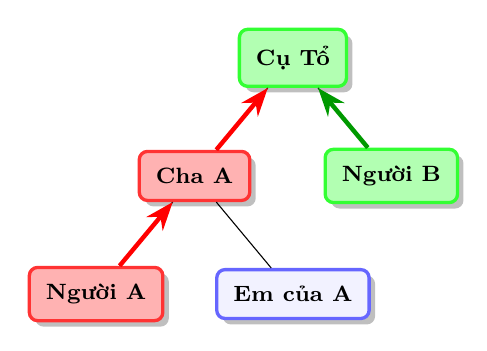
\begin{tikzpicture}[level distance=1.5cm, sibling distance=2.5cm]
        	% Tô màu toàn bộ đường đi từ A lên Root và B lên Root
        	\node (root) [person, pathA, pathB] {Cụ Tổ}
        	child { node (c1) [person, pathA] {Cha A} 
        		child { node (a) [person, pathA] {Người A} }
        		child { node (s1) [person] {Em của A} }
        	}
        	child { node (b) [person, pathB] {Người B} };
        	
        	\draw[line, red, ultra thick] (a) -- (c1);
        	\draw[line, red, ultra thick] (c1) -- (root);
        	\draw[line, green!60!black, ultra thick] (b) -- (root);
        	
        \end{tikzpicture}
    \end{minipage}      
    \caption{Mã giả và hình vẽ minh hoạ cho pha 1 của thuật toán.}
    \label{fig:LCAPhase1}
\end{figure}

\vspace*{-\baselineskip}
\textbf{\textit{Pha thứ hai: Xác định Tổ tiên chung gần nhất (LCA).}}
\begin{itemize}
    \item Mục tiêu của pha: Tìm ra nút chung đầu tiên mà cả hai đối tượng $A$ và $B$ cùng thuộc về nhánh hậu duệ của nút đó.
    \item Phương pháp thực hiện: Ta thực hiện phép so sánh hai tập $P_A$ và $P_B$ đã có được từ pha thứ nhất, cụ thể:
    \begin{itemize}
        \item So sánh hai danh sách $P_A$ và $P_B$ từ vị trí nút gốc (đầu danh sách).
        \item Nút cuối cùng trùng khớp trong cả hai danh sách trước khi đường đi rẽ nhánh chính là LCA cần tìm.
    \end{itemize}
    \item Về độ phức tạp: Độ phức tạp thời gian là $O(K)$, với $K = \min(h_A, h_B)$, phép so sánh được thực hiện trực tiếp trên địa chỉ bộ nhớ thay vì so sánh chuỗi.
\end{itemize}

\begin{figure}[H]
	\vspace*{-\baselineskip}
    \centering
    \begin{minipage}{0.50\textwidth}
        \begin{algorithm}[H]
        	\footnotesize
            \caption{DetermineRelationship (A, B)} \label{alg:DetermineRelationship}
            \begin{algorithmic}
                \State Đặt PathA = GetPathToRoot(A)
                \State Đặt PathB = GetPathToRoot(B)
                \For{$i$ from $0$ to $\min(h_A,h_B)$} 
                    \If {$PathA_i$ trùng $PathB_i$}
                        \State Đặt $\text{LCAIndex}=i$
                    \Else \ \textbf{break}
                    \EndIf
                \EndFor
                \If{$\text{LCAIndex}=-1$} \State \Return Không cùng huyết thống
                    \Else \ \Return LCAIndex
                \EndIf
            \end{algorithmic}
        \end{algorithm}
    \end{minipage}%
    \hfill
    \begin{minipage}{0.50\textwidth}
        \centering
        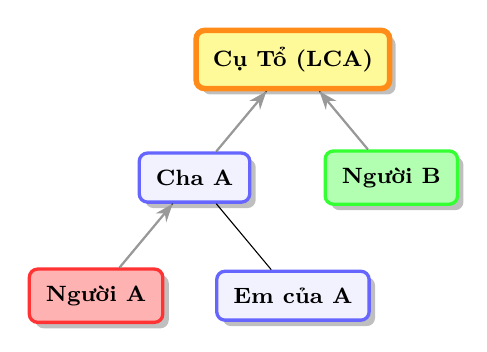
\begin{tikzpicture}[level distance=1.5cm, sibling distance=2.5cm]
        	% Chỉ tô đậm LCA
        	\node (root) [person, LCA] {Cụ Tổ (LCA)}
        	child { node (c1) [person] {Cha A} 
        		child { node (a) [person, pathA] {Người A} }
        		child { node (s1) [person] {Em của A} }
        	}
        	child { node (b) [person, pathB] {Người B} };
        	
        	\draw[line] (a) -- (c1);
        	\draw[line] (c1) -- (root);
        	\draw[line] (b) -- (root);
        \end{tikzpicture}
    \end{minipage}
    \caption{Mã giả và hình vẽ minh hoạ cho pha 2 của thuật toán}
    \label{fig:LCAPhase2}
    \vspace*{-\baselineskip}
\end{figure}


\textbf{\textit{Pha thứ ba: Tính toán véc-tơ khoảng cách.}}
\begin{itemize}
	\item Mục tiêu của pha: Định lượng khoảng cách thế hệ giữa các đối tượng và tổ tiên chung để làm cơ sở cho việc phân giải danh xưng.
	\item Phương pháp thực hiện: Gọi $d_A$ là khoảng cách thế hệ từ $LCA$ đến $A$. Gọi $d_B$ là khoảng cách thế hệ từ $LCA$ đến $B$. Lúc này, ta có một cặp tọa độ $(d_A, d_B)$ phản ánh cấp bậc của hai người, làm tiền đề cho pha cuối cùng.
	\item Về độ phức tạp: Vì mảng đường đi chứa tuần tự các đỉnh từ Gốc đến nút đích, khoảng cách $d$ được chứng minh bằng công thức toán học tuyệt đối: $d = (M - 1) - T$ với $M$ là chiều dài mảng và $T$ là vị trí của LCA. Vậy độ phức tạp thời gian và không gian cho pha này chỉ là $O(1)$.
\end{itemize}

\textbf{\textit{Pha cuối cùng: Phân giải danh xưng}}
\begin{itemize}
	\item Mục tiêu của pha: Chuyển đổi các giá trị toán học $(d_A, d_B)$ thành tên gọi quan hệ họ hàng theo quy chuẩn văn hóa.
	\item Phương pháp thực hiện: Sử dụng cấu trúc điều kiện để ánh xạ cặp $(d_A, d_B)$ vào ma trận danh xưng, cụ thể:
	
	\begin{center}
		\small
		\setlength{\tabcolsep}{4pt}
		\renewcommand{\arraystretch}{1.2}
		\begin{longtable}{
				|>{\centering\arraybackslash}m{2.2cm}|
				>{\centering\arraybackslash}m{3.2cm}|
				>{\centering\arraybackslash}m{3.2cm}|
				>{\arraybackslash}m{6.2cm}|
			}
			\hline
			\textbf{Tọa độ} $(dA,dB)$ & 
			\textbf{Quan hệ của B đối với A} & 
			\textbf{Quan hệ của A đối với B} & 
			\textbf{Giải thích Logic} \\ 
			\hline
			\endfirsthead
			
			\hline
			\textbf{Tọa độ} $(dA,dB)$ & 
			\textbf{Quan hệ của B đối với A} & 
			\textbf{Quan hệ của A đối với B} & 
			\textbf{Giải thích Logic} \\ 
			\hline
			\endhead
			
			\hline
			\multicolumn{4}{r}{\textit{Còn tiếp}} \\
			\endfoot
			
			\hline
			\endlastfoot
			
			$(k,0)$      & Tổ tiên đời thứ $k$                & Hậu duệ đời thứ $k$                & $B \equiv L$, $B$ là gốc của nhánh chứa $A$. \\ \hline
			$(0,k)$      & Hậu duệ đời thứ $k$                & Tổ tiên đời thứ $k$                & $A \equiv L$, $A$ là gốc của nhánh chứa $B$. \\ \hline
			$(k,k)$      & Anh/Chị/Em họ đời $k-1$           & Anh/Chị/Em họ đời $k-1$           & Chung tổ tiên cách đây $k$ thế hệ. \\ \hline
			$(1,2)$      & Bác/Cô/Chú/Dì                      & Cháu (gọi bằng Bác/Chú...)         & $B$ là con của anh/chị/em với $A$. \\ \hline
			$(2,1)$      & Cháu (gọi bằng Bác/Chú...)         & Bác/Cô/Chú/Dì                      & $A$ là con của anh/chị/em với $B$. \\ \hline
			$(1,k)$ với $k>2$ & Cụ/Kỵ (nhánh bàng hệ)          & Chắt/Chút (nhánh bàng hệ)          & $B$ là hậu duệ xa của anh/chị/em với $A$. \\ \hline
			$(dA,dB)$    & Họ hàng tổng quát                  & Họ hàng tổng quát                  & Cách nhau tổng $dA+dB$ bậc thế hệ. \\ \hline
			
		\end{longtable}
	\end{center}
\end{itemize}

\vspace*{-2\baselineskip}

\subsubsection{Thuật toán truy vấn theo danh xưng}

Một bài toán khác được đặt ra ngược với bài toán được xác định ở Mục \ref{sssec:lca1}, đó là tìm người theo quan hệ, nghĩa là: cho một người xác định và quan hệ (bố mẹ/ông bà/cô chú/...), ta cần phải tìm được một (hoặc nhiều) người có quan hệ đó với người đã xác định. Hệ thống tận dụng tính đối ngẫu của thuật toán LCA trước đó. Thay vì tìm tọa độ từ hai nút, ta sẽ cố định tọa độ $(d_A, d_B)$ dựa trên danh xưng tiếng Việt và thực hiện truy vết ngược từ con trỏ \texttt{pParent} kết hợp duyệt nhánh ngang \texttt{pNextSibling} để trả về kết quả cần thiết. Cụ thể, thuật toán này trải qua ba pha như sau:

\textbf{\textit{Pha thứ nhất: Xác định tổ tiên.}}
\begin{itemize}
	\item Mục tiêu của pha: Tìm ra nút tổ tiên chung ($L$).
	\item Phương pháp thực hiện: Từ nút $A$, di chuyển qua con trỏ pParent đúng $d_A$ lần. Ví dụ: Tìm ``Chú'' thì $d_A = 2$. Từ $A$, ta cần leo lên ``Bố'' ($d=1$), rồi sau đó lên ``Ông nội'' ($d=2$). Nút Ông nội chính là $L$.
	\item Về độ phức tạp: Độ phức tạp thời gian là $O(d_A)$, vì chỉ đi theo một đường thẳng nên rất nhanh.
\end{itemize}

\begin{figure}[htbp]
	\vspace*{-\baselineskip}
	\begin{algorithm}[H]
		\footnotesize
		\caption{FindAncestor(startP, dA)}
		\begin{algorithmic}[1]
			\State temp $\gets$ startP
			\For{$i=1$ \to $dA$}
			\If{temp.parent $\neq$ NULL}
			\State temp $\gets$ temp.parent
			\Else \ \Return NULL \Comment{Không đủ độ sâu thế hệ}
			\EndIf
			\EndFor
			\State\ \Return temp
		\end{algorithmic}
	\end{algorithm}
	\vspace*{-\baselineskip}
	\caption{Mã giả mô tả pha thứ nhất của thuật toán truy vấn theo danh xưng}
	\vspace*{-\baselineskip}
\end{figure}


\textbf{\textit{Pha thứ hai: Duyệt và lọc đối tượng.}}
\begin{itemize}
	\item Mục tiêu của pha: Thu thập được những người phù hợp.
	\item Phương pháp thực hiện: Từ tổ tiên $L$, ta cần tìm các hậu duệ ở mức thế hệ $d_B$ thỏa mãn các điều kiện về giới tính và thứ tự. Ta sẽ sử dụng phương pháp duyệt theo chiều rộng (BFS) để tìm tất cả các nút cách $L$ đúng $d_B$ bậc.
	\item Về độ phức tạp: Độ phức tạp thời gian là $O(S)$, với $S$ là số lượng anh/em/con/cháu trong nhánh đang xét đó.
\end{itemize}
%Mã giả mô tả thuật toán của pha ở hình \ref{fig:Rel1}.
\begin{figure}[htbp]
	\vspace*{-\baselineskip}
	\centering
	\begin{algorithm}[H]
		\footnotesize
		\caption{Thuật toán thu thập ứng viên cùng thế hệ}
		\begin{algorithmic}[1]
			% Hàm thu thập tất cả các node cách gốc một khoảng dB
			\Function{CollectCandidates}{root, dB}
			\State Cands $\gets \emptyset$ \Comment{Khởi tạo tập ứng viên rỗng}
			
			\If{$dB = 0$}
			\State \Return \{root\} \Comment{Nếu khoảng cách = 0, trả về chính gốc}
			\EndIf
			
			% Thủ tục đệ quy để duyệt cây
			\Procedure{DuyetTang}{curr, depth}
			\If{curr = NULL} 
			\State \Return \Comment{Trường hợp cơ sở: không có node để xử lý}
			\EndIf
			
			\If{depth = dB}
			\State Cands $\gets$ Cands $\cup$ \{curr\} \Comment{Thêm node hiện tại vào tập ứng viên}
			\State \Return \Comment{Dừng duyệt sâu hơn}
			\EndIf
			
			\State \Call{DuyetTang}{curr.firstChild, depth + 1} \Comment{Duyệt node con đầu tiên (xuống sâu hơn)}
			
			\State t $\gets$ curr.firstChild \Comment{Bắt đầu duyệt các node anh em}
			\While{t $\neq$ NULL \textbf{and} t.nextSibling $\neq$ NULL}
			\State t $\gets$ t.nextSibling \Comment{Chuyển sang node anh em kế tiếp}
			\State \Call{DuyetTang}{$t$, $depth + 1$} \Comment{Duyệt cây con của node anh em này}
			\EndWhile
			\EndProcedure
			
			\State \Call{DuyetTang}{root, 0} \Comment{Bắt đầu duyệt từ gốc ở độ sâu 0}
			\State \Return $Cands$ \Comment{Trả về tất cả các ứng viên đã thu thập được}
			\EndFunction
		\end{algorithmic}
	\end{algorithm}
	\vspace*{-\baselineskip}
	\caption{Mã giả mô tả pha thứ hai của thuật toán truy vấn theo danh xưng}
	\label{fig:Rel1}
\end{figure}
\textbf{\textit{Pha thứ ba: Phân giải danh xưng cụ thể.}}
\begin{itemize}
	\item Mục tiêu của pha: Áp dụng những ràng buộc đã có để đưa ra người cần tìm kiếm.
	\item Phương pháp thực hiện: Đây là lúc áp dụng các ràng buộc mà nhóm đã thiết kế trong struct \texttt{Person}, cụ thể là phân giải theo ``Giới tính'' và ``Thứ tự''. Cụ thể:
	\begin{itemize}
		\item Theo Giới tính: Nếu yêu cầu là ``Cô'', lọc những người có \texttt{gender} là ``Nữ''.
		\item Theo Thứ tự: Dựa vào con trỏ \texttt{pNextSibling}. Nếu người đó nằm phía trước Cha của A trong danh sách anh em, đó là ``Bác'', ngược lại là ``Chú''.
	\end{itemize}
\end{itemize}

Tổng quát, thuật toán chung của ta vẫn tiệm cận mức $O(H)$, rõ ràng là hiệu quả hơn nhiều so với việc quét toàn bộ người trong gia phả. Ngoài ra, thuật toán này còn có ưu điểm là xử lý được trường hợp đa kết quả (ví dụ: tìm ``Chú'' có thể cho ra nhiều người, việc tìm người cụ thể do người dùng quyết định).

Ngoài ra, vì cấu trúc LCRS truyền thống chỉ lưu trữ các thực thể có quan hệ huyết thống trực tiếp, khiến các thành viên nữ (vợ) trở thành ``điểm mù'' (nghĩa là, không thể thực hiện bất kỳ chức năng nào của hệ thống trên những người này) của giải thuật duyệt cây. Vì vậy, giải pháp cho điều này là sử dụng cơ chế Proxy Node (Nút đại diện). Khi truy vấn ``Mẹ'', hệ thống thực hiện tìm kiếm gián tiếp: \texttt{Mother(A) = Spouse(Parent(A))}, cụ thể:
\begin{itemize}
	\item Hệ thống xác định nút Cha của A (là nút $P$ trong cây).
	\item Sau đó, hệ thống truy xuất vào thuộc tính \texttt{spouseName} (vợ) của nút $P$.
\end{itemize}

Cách làm này giữ cho cây luôn là cây đơn gốc (single-root tree), giúp các thuật toán duyệt đệ quy và LCA luôn đạt độ phức tạp tối ưu nhất.

\subsubsection{Thuật toán lưu trữ và phục hồi}

Trong môi trường quản lý dữ liệu bằng con trỏ động, địa chỉ bộ nhớ của các thực thể (\texttt{Person}) chỉ có giá trị nội hàm trong phiên làm việc hiện tại của RAM. Để đảm bảo tính bền vững của dữ liệu, nhóm áp dụng kỹ thuật Tuần tự hóa nhị phân (Binary Serialization) kết hợp với thuật toán Phẳng hóa đồ thị cây.

\textbf{\textit{Cấu trúc Bản ghi tĩnh trung gian (\texttt{PersonRecord})}}

Để khắc phục nhược điểm của chuỗi động \texttt{std::string}, chương trình định nghĩa một cấu trúc \texttt{PersonRecord} kích thước cố định, sử dụng mảng ký tự tĩnh (\texttt{char[]}). Các liên kết con trỏ LCRS (\texttt{pParent}, \texttt{pFirstChild}, \texttt{pNextSibling}) được thay thế hoàn toàn bằng định danh số nguyên là \texttt{id} (mã cá nhân) và \texttt{parentId} (mã của nút cha).

\textbf{\textit{Giải thuật Ghi tệp (Phẳng hóa cây LCRS)}}
\begin{itemize}
	\item Hệ thống sử dụng thuật toán duyệt cây Tiền thứ tự (Pre-order Traversal) thông qua hàm đệ quy \texttt{FlattenTree}.
	\item Tại mỗi nút, dữ liệu được sao chép an toàn (sử dụng \texttt{strncpy} để chống tràn bộ đệm) sang cấu trúc \texttt{PersonRecord} và đẩy vào một mảng động \texttt{std::vector}.
	\item Thay vì ghi tuần tự từng cá nhân, chương trình áp dụng kỹ thuật Block I/O: tính toán tổng dung lượng của mảng và sử dụng phương thức \texttt{write()} để đổ toàn bộ khối dữ liệu từ RAM xuống tệp \texttt{.dat} trong một chu kỳ ghi duy nhất.
\end{itemize}

\begin{figure}[htbp]
	\vspace*{-\baselineskip}
	\centering
	\begin{algorithm}[H]
		\footnotesize
		\caption{Hàm FlattenTree}
		\begin{algorithmic}[1]
			\Require currentNode, recordArray
			
			\State \Comment{Điều kiện dừng đệ quy}
			\If{currentNode là RỖNG}
			\Return
			\EndIf
			
			\State \Comment{1. Chuyển đổi Node động thành Bản ghi tĩnh}
			\State Tạo NewRecord
			\State NewRecord.id = currentNode.id
			
			\If{currentNode có Cha}
			\State NewRecord.parentId = currentNode.parent.id
			\Else
			\State NewRecord.parentId = 0  \Comment{0 ám chỉ đây là Cụ Tổ (Gốc)}
			\EndIf
			
			\State Chép các thông tin (Tên, Năm sinh...) từ Node sang Bản ghi
			
			\State \Comment{2. Lưu vào mảng}
			\State Thêm NewRecord vào recordArray
			
			\State \Comment{3. Đệ quy đi tiếp xuống nhánh Con và nhánh Em}
			\State FlattenTree(currentNode.firstChild, recordArray)
			\State FlattenTree(currentNode.nextSibling, recordArray)
		\end{algorithmic}
	\end{algorithm}
	\vspace*{-\baselineskip}
	\caption{Mã giả mô tả thuật toán phẳng hoá cây để lưu file}
	\vspace*{-\baselineskip}
\end{figure}


\textbf{\textit{Giải thuật Đọc tệp và Tái cấu trúc}}

Quá trình phục hồi dữ liệu từ tệp nhị phân được tối ưu hóa ở mức cao nhất nhằm tránh việc tìm kiếm lặp lại:
\begin{enumerate}
	\item Chương trình đọc toàn bộ khối dữ liệu từ tệp lên một mảng \texttt{PersonRecord} trên RAM.
	\item Khởi tạo một Bảng băm (Hash Map) sử dụng cấu trúc \texttt{std::unordered\_map<int, Person*>} để thiết lập quan hệ ánh xạ giữa \texttt{id} nguyên thủy và địa chỉ bộ nhớ động vừa được cấp phát.
	\item Khi duyệt qua từng bản ghi, hệ thống tạo mới một đối tượng \texttt{Person} và sử dụng \texttt{parentId} để tra cứu trực tiếp địa chỉ người cha trong Bảng băm. Thao tác tra cứu này đạt độ phức tạp thời gian $O(1)$, cho phép liên kết con trỏ ngay lập tức thông qua hàm \texttt{AddChild} mà không cần duyệt lại cây LCRS.
	\item Hệ thống tự động cập nhật lại biến đếm ID toàn cục (\texttt{global\_id\_counter}) dựa trên mức ID lớn nhất trong tệp để đảm bảo tính duy nhất cho các phiên nhập liệu tiếp theo.
\end{enumerate}

\textbf{\textit{Đánh giá thuật toán}}

Cả hai tiến trình Serialization và Deserialization đều đạt độ phức tạp thời gian $O(N)$ và không gian $O(N)$, với $N$ là tổng số thành viên trong gia phả. Việc kết hợp Block I/O và Hash Map giúp giải thuật xử lý mượt mà dữ liệu quy mô hàng vạn thực thể mà không gây ra tình trạng tràn ngăn xếp (Stack Overflow) hay nghẽn cổ chai truy xuất đĩa.

\subsubsection{Thuật toán thống kê dòng họ}

Thuật toán thống kê cung cấp cái nhìn tổng quan về quy mô và cấu trúc của dòng họ thông qua các chỉ số định lượng, nhằm giúp người quản trị nắm bắt được tổng số thành viên (bao gồm cả huyệt thống và phu nhân), sự phân bổ giới tính, độ dài thế hệ (số đời), và tình trạng sinh tồn của các cá nhân trong gia phả.

Do gia phả được lưu trữ dưới dạng cây LCRS, việc thống kê được thực hiện tối ưu nhất bằng phương pháp Duyệt cây theo chiều sâu (DFS) kết hợp với kỹ thuật đệ quy. Mỗi khi đi qua một nút ($Node$), hệ thống sẽ thực hiện kiểm tra các thuộc tính của thực thể Person và cập nhật vào cấu trúc dữ liệu \texttt{FamilyStats}.

Các bước cụ thể như sau:
\begin{itemize}
	\item Bước 1: Tạo một cấu trúc lưu trữ \texttt{FamilyStats} với các biến đếm (tổng số, nam, nữ, phu nhân, tử vong) và một mảng \texttt{genDistribution} để lưu số lượng thành viên của từng đời.
	\item Bước 2: Đệ quy xử lý nút hiện tại. Tăng biến \texttt{totalMembers}; Kiểm tra gender: Nếu là ``Nam'' tăng \texttt{maleCount}, nếu ``Nu'' tăng \texttt{femaleCount}; kiểm tra \texttt{spouseName}: Nếu khác ``None'' hoặc ``N/A'', tăng \texttt{totalSpouses} (thống kê dâu/rể); Kiểm tra \texttt{deathDay}: Nếu khác ``N/A'', tăng \texttt{deceasedCount}; Cập nhật thế hệ: Sử dụng tham số \texttt{level} để tăng giá trị tại \texttt{genDistribution[level]} và cập nhật \texttt{maxGen = max(maxGen, level)}.
	\item Bước 3: Lan toả đệ quy. Gọi đệ quy xuống con đầu tiên và gọi đệ quy sang anh em kế cận.
\end{itemize}

\textbf{\textit{Phân tích độ phức tạp}}

\begin{itemize}
	\item Độ phức tạp thời gian: $O(N)$, với $N$ là tổng số nút trong cây gia phả. Thuật toán chỉ đi qua mỗi nút đúng một lần duy nhất.
	\item Độ phức tạp không gian: $O(H)$, với $H$ là chiều cao của cây (tương ứng với số đời), do sử dụng ngăn xếp đệ quy trong quá trình duyệt.
\end{itemize}

    \section{CHƯƠNG TRÌNH VÀ KẾT QUẢ}
    \subsection{Tổ chức chương trình}
\subsubsection{Kiến trúc tổng thể của chương trình}
Hệ thống được thiết kế và xây dựng dựa trên mô hình Lập trình theo mô-đun (module). Thay vì tập trung toàn bộ mã nguồn vào một tệp duy nhất, chương trình được phân rã thành các mô-đun độc lập dựa trên \textit{nguyên lý Phân tách trách nhiệm}.

Cách tiếp cận này đảm bảo hệ thống đạt được độ gắn kết cao bên trong từng mô-đun và độ phụ thuộc thấp giữa các mô-đun với nhau, tạo tiền đề thuận lợi cho việc kiểm thử, gỡ lỗi và mở rộng tính năng trong tương lai.
\subsubsection{Cấu trúc tệp tin và phân rã chức năng}

Mã nguồn của đồ án được tổ chức thành 6 thành phần cốt lõi, bao gồm 1 tệp tiêu đề cơ sở, 4 cặp module logic (\texttt{.h} và \texttt{.cpp}) và một tệp điều khiển trung tâm. Chi tiết chức năng của từng tệp được quy định như sau:
\begin{enumerate}[label*=(\alph*)]
	\item \texttt{DataStructures.h}: Định nghĩa cấu trúc nút LCRS, bản ghi và biến toàn cục, đảm bảo nhất quán kiểu dữ liệu giữa các mô-đun.
	\item \texttt{TreeManager.h/.cpp}: Thao tác trực tiếp trên RAM; khởi tạo biến toàn cục; quản lý vòng đời nút (cấp phát, giải phóng, truy xuất).
	\item \texttt{SearchEngine.h/.cpp}: Xử lý truy vấn, kiểm soát trùng lặp; duyệt DFS để tìm kiếm; cung cấp giao diện chọn thực thể.
	\item \texttt{Relationship.h/.cpp}: Giải quyết bài toán đồ thị gia phả; tìm tổ tiên chung (LCA); đổi tọa độ thế hệ sang danh xưng và ngược lại.
	\item \texttt{FileHandler.h/.cpp}: Quản lý I/O với ổ cứng; tuần tự hóa cây LCRS thành mảng, ghi/đọc file nhị phân; hỗ trợ nhập từ file văn bản, xử lý lỗi dòng.
	\item \texttt{main.cpp}: Khởi chạy, tạo dữ liệu mẫu, điều hướng sự kiện và xử lý lỗi nhập.
\end{enumerate}

\begin{figure}[h!]
	\begin{tikzpicture}[
		box/.style={draw, rounded corners=6pt, minimum width=2.8cm, minimum height=1cm, align=center, font=\small},
		 >={Stealth},
		mainbox/.style={box, fill=yellow!30, draw=yellow!50!black, very thick},
		bluebox/.style={box, fill=blue!20, draw=blue!50!black, very thick},
		redbox/.style={box, fill=red!20, draw=red!60!black, very thick},
		arrow/.style={->, very thick},
		darrow/.style={<->, very thick},
		dottedarrow/.style={->, dotted, very thick},
		]
		
		% Main
		\node[mainbox] (main) at (0,0) {main.cpp};
		
		% Middle layer (FIXED positions)
		\node[bluebox] (search) at (-6,-2.5) {SearchEngine};
		\node[bluebox] (file)   at (-2,-2.5) {FileHandler};
		\node[bluebox] (rel)    at (2,-2.5)  {Relationship};
		\node[bluebox] (tree)   at (6,-2.5)  {TreeManager};
		
		% Bottom
		\node[redbox] (data) at (0,-5) {DataStructures};
		
		% Arrows
		\draw[arrow] (main) -- (search);
		\draw[arrow] (main) -- (file);
		\draw[arrow] (main) -- (rel);
		\draw[arrow] (main) -- (tree);
		
		\draw[darrow] (search) -- (file);
		\draw[darrow] (file) -- (rel);
		\draw[darrow] (rel) -- (tree);
		
		\draw[dottedarrow] (search) -- (data);
		\draw[dottedarrow] (file) -- (data);
		\draw[dottedarrow] (rel) -- (data);
		\draw[dottedarrow] (tree) -- (data);
		\draw[dottedarrow] (main) -- (data);
		
		\node[draw, rectangle, right=2cm of data, align=right, scale=0.8] (legend) {
			\begin{tikzpicture}[scale=0.9]
				\draw[darrow] (0,0) -- (1,0) node[right]{Hỗ trợ};
				\draw[arrow] (0,-0.5) -- (1,-0.5) node[right]{Điều khiển};
				\draw[dottedarrow] (0,-1) -- (1,-1) node[right]{Dựa trên nền tảng của};
			\end{tikzpicture}
		};
		
	\end{tikzpicture}
	\caption{Sơ đồ mô tả cấu trúc chương trình và các tệp tin}
\end{figure}

\begin{sidewaysfigure}
	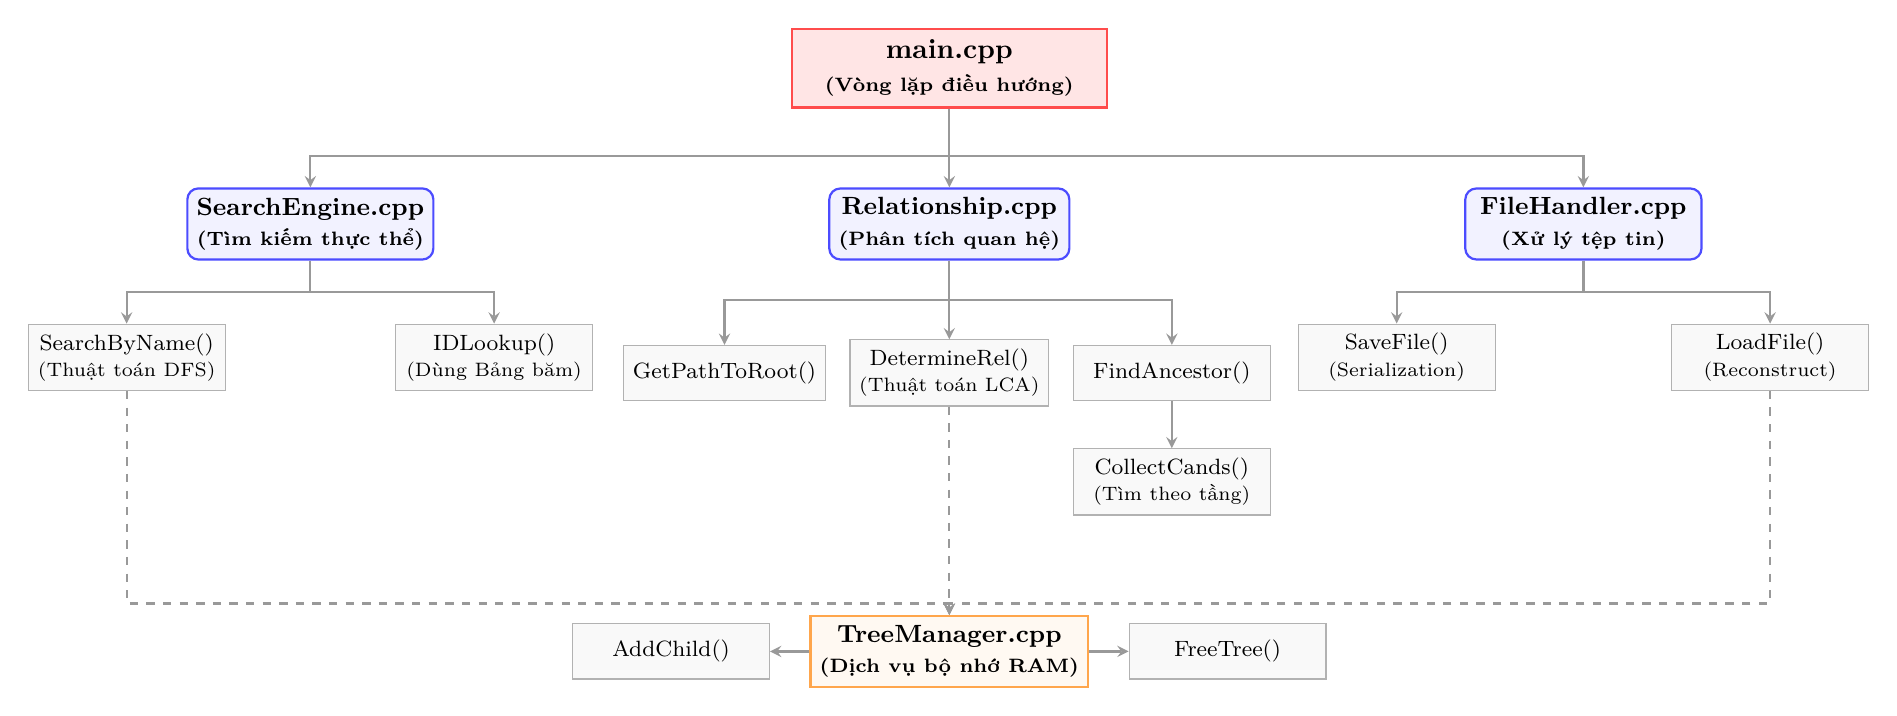
\begin{tikzpicture}[
		node distance=1cm,
		block/.style={rectangle, draw=blue!70, fill=blue!5, thick, minimum width=3cm, minimum height=0.8cm, align=center, font=\bfseries\small, rounded corners},
		subblock/.style={rectangle, draw=gray!60, fill=gray!5, minimum width=2.5cm, minimum height=0.7cm, align=center, font=\footnotesize},
		mainblock/.style={rectangle, draw=red!70, fill=red!10, thick, minimum width=4cm, minimum height=1cm, align=center, font=\bfseries},
		managerblock/.style={rectangle, draw=orange!70, fill=orange!5, thick, minimum width=3.5cm, minimum height=0.8cm, align=center, font=\bfseries\small},
		arrow/.style={-stealth, thick, draw=gray!80}
		]
		
		% --- TẦNG 1: ĐIỀU KHIỂN ---
		\node[mainblock] (main) {main.cpp \\ \scriptsize (Vòng lặp điều hướng)};
		
		% --- TẦNG 2: MODULE LOGIC (Dàn hàng ngang rộng) ---
		\node[block, below=of main] (rel) {Relationship.cpp \\ \scriptsize (Phân tích quan hệ)};
		\node[block, left=5cm of rel] (search) {SearchEngine.cpp \\ \scriptsize (Tìm kiếm thực thể)};
		\node[block, right=5cm of rel] (file) {FileHandler.cpp \\ \scriptsize (Xử lý tệp tin)};
		
		% --- TẦNG 3: CÁC HÀM CHI TIẾT ---
		% Nhánh Search
		\node[subblock, below left=0.8cm and -0.5cm of search] (dfs) {SearchByName() \\ \scriptsize (Thuật toán DFS)};
		\node[subblock, below right=0.8cm and -0.5cm of search] (hash) {IDLookup() \\ \scriptsize (Dùng Bảng băm)};
		
		% Nhánh Relationship
		\node[subblock, below=1cm of rel] (lca) {DetermineRel() \\ \scriptsize (Thuật toán LCA)};
		\node[subblock, left=0.3cm of lca] (path) {GetPathToRoot()};
		\node[subblock, right=0.3cm of lca] (anc) {FindAncestor()};
		\node[subblock, below=0.6cm of anc] (coll) {CollectCands() \\ \scriptsize (Tìm theo tầng)};
		
		% Nhánh File
		\node[subblock, below left=0.8cm and -0.4cm of file] (save) {SaveFile() \\ \scriptsize (Serialization)};
		\node[subblock, below right=0.8cm and -0.4cm of file] (load) {LoadFile() \\ \scriptsize (Reconstruct)};
		
		% --- TẦNG 4: TREE MANAGER (Dùng chung) ---
		\node[managerblock, below=4.5cm of rel] (manager) {TreeManager.cpp \\ \scriptsize (Dịch vụ bộ nhớ RAM)};
		\node[subblock, left=0.5cm of manager] (add) {AddChild()};
		\node[subblock, right=0.5cm of manager] (free) {FreeTree()};
		
		% --- KẾT NỐI MŨI TÊN ---
		% Main gọi 3 module chính
		\draw[arrow] (main.south) -- (rel.north);
		\draw[arrow] (main.south) -- ++(0,-0.6) -| (search.north);
		\draw[arrow] (main.south) -- ++(0,-0.6) -| (file.north);
		
		% Nội bộ Search
		\draw[arrow] (search.south) -- ++(0,-0.4) -| (dfs.north);
		\draw[arrow] (search.south) -- ++(0,-0.4) -| (hash.north);
		
		% Nội bộ Relationship
		\draw[arrow] (rel.south) -- (lca.north);
		\draw[arrow] (rel.south) -- ++(0,-0.5) -| (path.north);
		\draw[arrow] (rel.south) -- ++(0,-0.5) -| (anc.north);
		\draw[arrow] (anc.south) -- (coll.north);
		
		% Nội bộ File
		\draw[arrow] (file.south) -- ++(0,-0.4) -| (save.north);
		\draw[arrow] (file.south) -- ++(0,-0.4) -| (load.north);
		
		% Tất cả đổ về TreeManager khi cần thao tác nút
		\coordinate (mid) at (0,-6.8);
		\draw[arrow, dashed] (dfs.south) |- (mid) -| (manager.north);
		\draw[arrow, dashed] (lca.south) -- (manager.north);
		\draw[arrow, dashed] (load.south) |- (mid) -| (manager.north);
		
		\draw[arrow] (manager.west) -- (add.east);
		\draw[arrow] (manager.east) -- (free.west);
		
	\end{tikzpicture}
	\caption{Sơ đồ cấu trúc các hàm chính của chương trình}
\end{sidewaysfigure}

Toàn bộ mã nguồn của chương trình quản lý gia phả có tại Phụ lục đính kèm theo báo cáo này.

\subsection{Ngôn ngữ cài đặt}

\subsubsection{Lý do sử dụng ngôn ngữ C++}
Dự án lựa chọn ngôn ngữ C++ làm ngôn ngữ lập trình chính để triển khai hệ thống bởi những lý do như sau:
\begin{itemize}
	\item Mô hình LCRS yêu cầu cấp phát bộ nhớ liên tục, C++ dùng new/delete để kiểm soát vòng đời của từng nút (Person) một cách chính xác, nhờ đó tối ưu hiệu suất.
	\item Dùng \texttt{std::string} thay vì mảng char giúp xử lý tên tiếng Việt an toàn, tránh tràn bộ đệm. \texttt{std::vector} cũng được dùng để lưu kết quả tìm kiếm, giúp mã nguồn ngắn gọn, rõ ràng.
	\item Nhờ struct/class, C++ mô hình hóa “Con người” tự nhiên với đầy đủ thuộc tính và quan hệ, đồng thời dễ dàng tách chương trình thành các tệp \texttt{.h} và \texttt{.cpp}.
\end{itemize}

\subsubsection{Môi trường phát triển và công cụ hỗ trợ}
\begin{itemize}
	\item Trình biên dịch: Sử dụng GCC (\texttt{g++}) tiêu chuẩn C++11 trở lên để hỗ trợ các tính năng hiện đại và đảm bảo tốc độ thực thi tối ưu.
	\item Hệ thống được phát triển trên các IDE phổ biến như \textit{Embarcadero Dev-C++} và \textit{Visual Studio}, tận dụng khả năng quản lý \textit{project} để liên kết các tệp tin mô-đun.
	\item Định dạng tệp lưu trữ: tệp nhị phân (.dat) dùng để lưu trữ trạng thái cây dưới dạng các struct tĩnh, đảm bảo tốc độ đọc/ghi nhanh và bảo mật dữ liệu cơ bản; tệp văn bản (\texttt{.txt}) Dùng để nhập liệu hàng loạt theo định dạng phân tách bằng dấu phẩy (CSV), giúp người dùng dễ dàng soạn thảo dữ liệu từ bên ngoài.
\end{itemize}

\subsection{Kết quả}
    
	% === PHỤ LỤC ===
	\appendix
	
	\renewcommand{\refname}{TÀI LIỆU THAM KHẢO}
	\newpage
\addcontentsline{toc}{section}{Tài liệu tham khảo}


\begin{thebibliography}{10}
	
	\bibitem{cormen2022}
	Cormen, T. H., Leiserson, C. E., Rivest, R. L., \& Stein, C. (2022). \textit{Introduction to algorithms} (4th ed.). MIT Press.
	
	\bibitem{dangthienbinh}
	Đặng Thiên Bình (n.d.). \textit{Bài giảng Cấu trúc dữ liệu}. Lưu hành nội bộ.
	
	\bibitem{chahelgupta}
	chahelgupta. (n.d.). \textit{DSA-Project-FamilyTree: C++ program for building and visualizing a hierarchical family tree}. GitHub. \url{https://github.com/chahelgupta/DSA-Project-FamilyTree}
	
	\bibitem{praveenmylavarapu}
	praveenmylavarapu. (n.d.). \textit{family-tree: A family tree program in C++ using n-ary tree}. GitHub. \url{https://github.com/praveenmylavarapu/family-tree}
	
	\bibitem{tenouk}
	tenouk. (n.d.). \textit{Constructing a very simple family structure tree using the C++ inheritance principles}. tenouk.com. \url{https://www.tenouk.com/cpluscodesnippet/cplusclassinheritancefamilytree.html}
	
	\bibitem{qnu2025}
	Trường Đại học Quy Nhơn. (2025). \textit{Mẫu code C++ cho cây nhị phân và cây gia phả}. Studocu. \url{https://www.studocu.vn/vn/document/dai-hoc-quy-nhon/li-luan-giang-day/mau-code-c-cho-cay-nhi-phan-va-cay-gia-pha-kcj/148579038}
	
	\bibitem{minhtc}
	homielab. (n.d.). \textit{Gia Phả OS (Gia Phả Open Source)}. Github. \url{https://github.com/homielab/giapha-os}
	
	\bibitem{wikipedia2025}
	Wikipedia contributors. (2025). \textit{Kinship}. Wikipedia, The Free Encyclopedia. \url{https://en.wikipedia.org/wiki/Kinship}
	
\end{thebibliography}
\end{document}